\section{RubberEdge Device}

\begin{figure}[h]
    \centering
    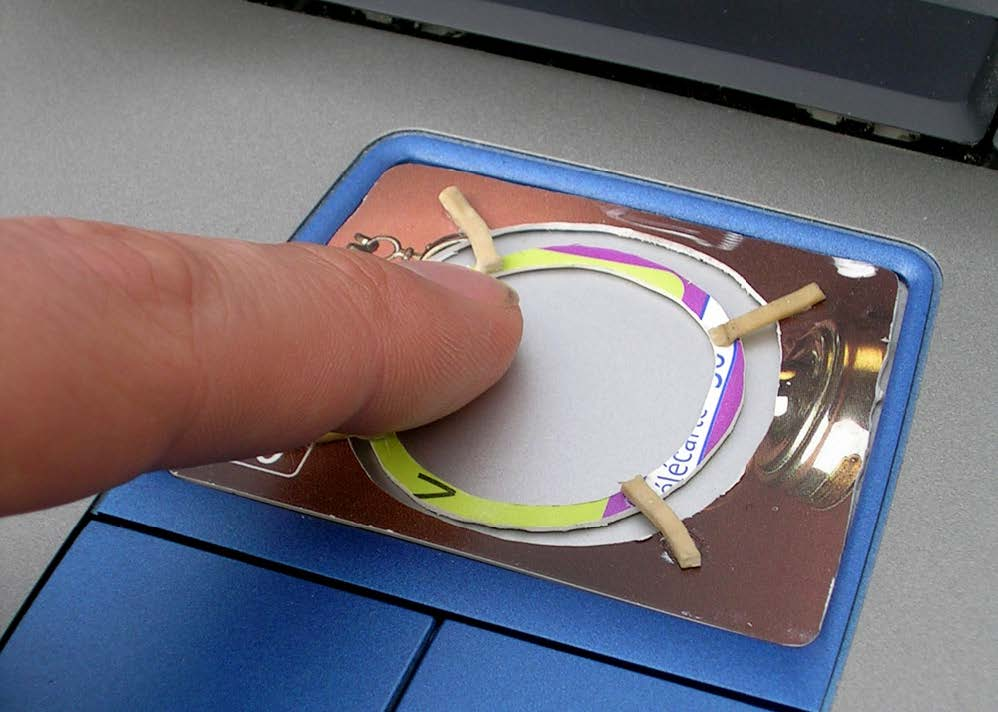
\includegraphics[width=0.9\columnwidth]{Existing}
    \caption{The RubberEdge interface from the previous study on RubberEdge \protect\cite{Casiez2007RubberEdge}}
    \label{fig:existing}
\end{figure}

This research paper aims to improve upon an existing RubberEdge implementation. The paper\cite{Casiez2007RubberEdge} that this research draws inspiration from only empirically examines their implementation of the RubberEdge as shown in Figure \ref{fig:existing}. The experimental results show in the paper were gathered with a Phantom Omni haptic device\cite{GeomagicOverview}, this apparatus mocked the feeling of RubberEdge to the participant. Although the interaction was not quite the same as it would be with a real touchpad, as the participant would not get the same feedback from physically pushing up against a ring over feeling some resistance. This research started with creating a RubberEdge apparatus using the existing design from the source paper.

\subsection{Interface Design}
The initial design called for a device which would sit neatly over a touchpad on a laptop. Measurements of the laptop's touchpad were 105mm x 80mm, after accounting for structural integrity of the edges of the interface, the design left a circular area with a 30mm radius, for the isotonic zone and around 7.5mm of radius for the elastic zone, the actual available area is less due to the collapsing spring arms of the final design. This left a usable isotonic area of 2827mm$^2$

In the first iteration of the design, an initial attempt at replicating the existing design was attempted by laser cutting an outer frame and inner ring out of acrylic. This design was abandoned in favour of a solution suggested by the mechanical technician that helped with the laser cutting and subsequent 3D printing. They suggested that a solution using spring arms might be an effective alternative, a design was quickly drafted, and cut from acrylic. The design showed promise but unfortunately, the acrylic material proved to be too rigid, and the spring arms would break under force.

\begin{figure}[h]
    \centering
    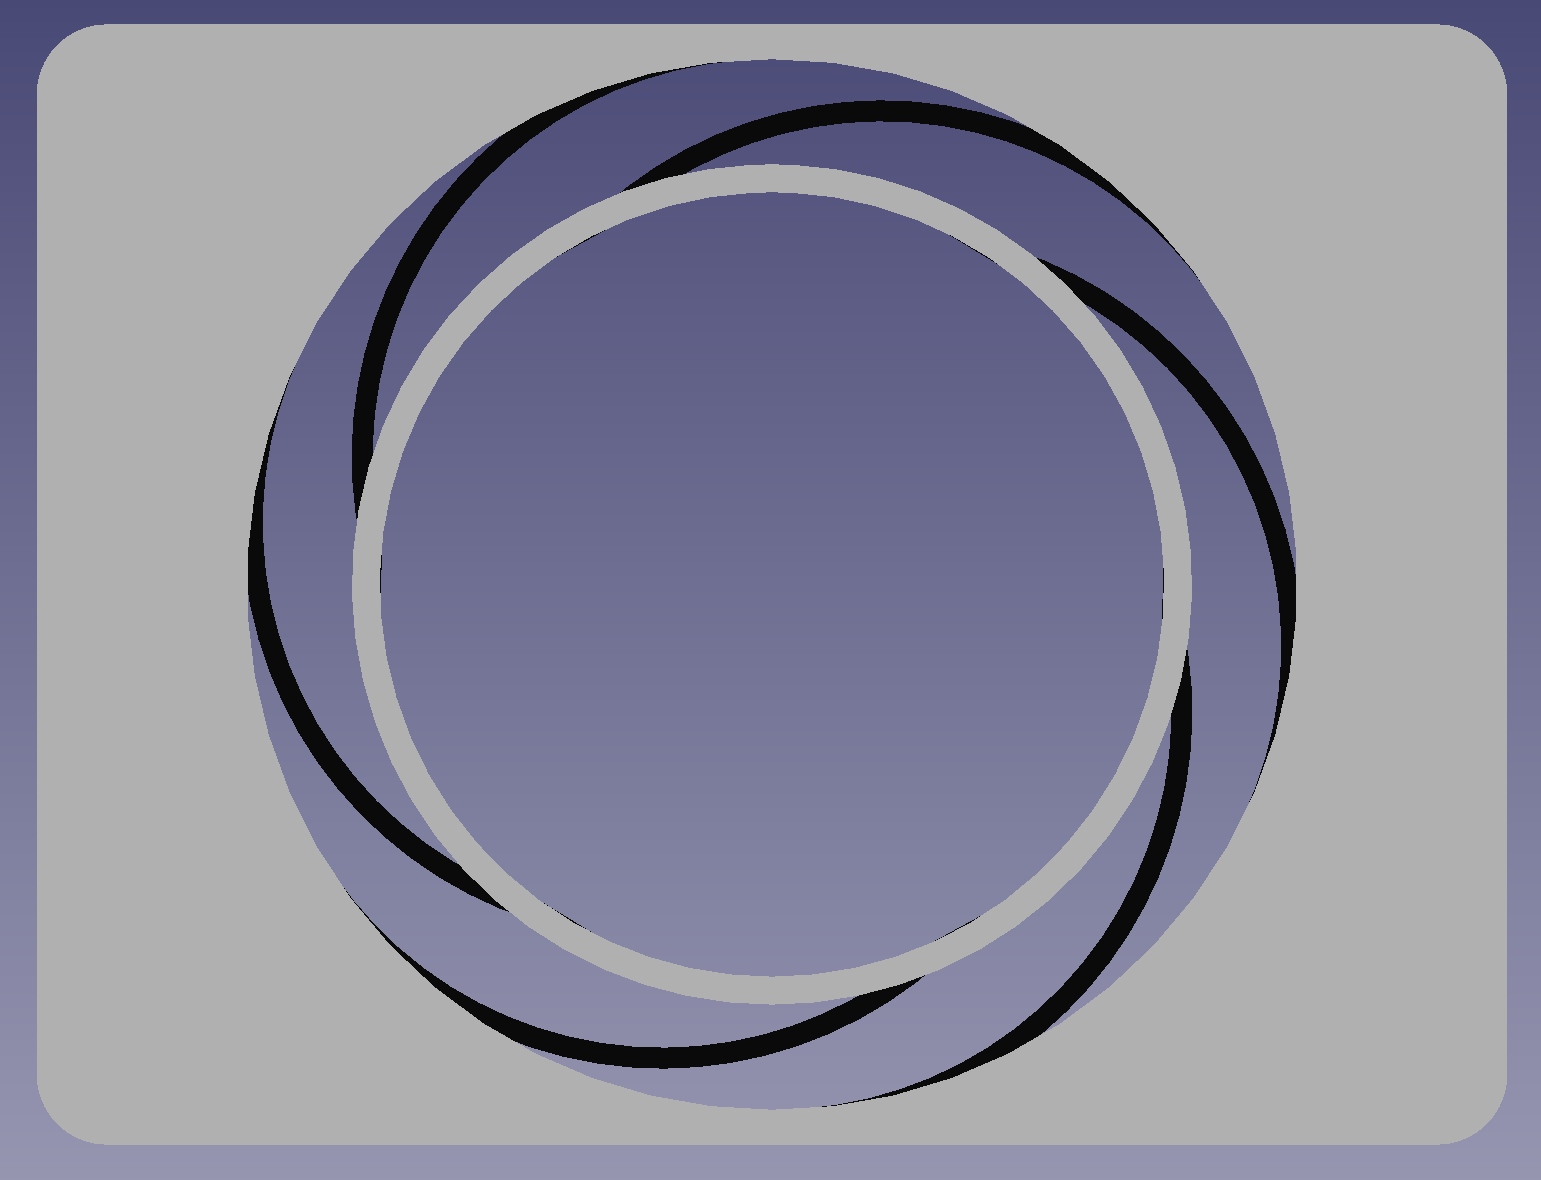
\includegraphics[width=0.9\columnwidth]{CADdesignV1}
    \caption{First design for the composite 3D printed RubberEdge interface.}
    \label{fig:cadv1}
\end{figure}

An alternative method of creating the interface was to use a composite 3D printer; this printer can blend multiple polymers to change the ply-ability of the plastic. A hybrid design was used where the outer frame and inner ring was printed with a rigid material, and the spring arms printed with an elastic type polymer, this design can be seen in Figure \ref{fig:cadv1}. The proprieties of the elastic material used are not freely available as the technology is proprietary to the manufacturer of the 3D printer, and material. The material is simply described as Shore 85, which only indicates the hardness of the material. Further tests should be conducted to evaluate the elasticity of the material to see if it falls in line with design guidelines present in this study\cite{Casiez2008TheDevice}.

\begin{figure}[h]
    \centering
    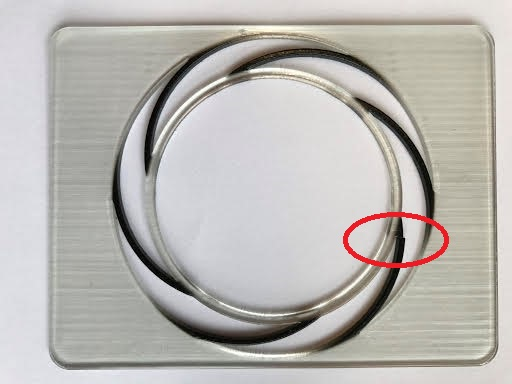
\includegraphics[width=0.9\columnwidth]{3Dprintv1}
    \caption{As shown in the red circle, a major problem of the first spring arm design was the spring arms breaking after a period of use.}
    \label{fig:3dprintv1}
\end{figure}

\begin{figure}[h]
    \centering
    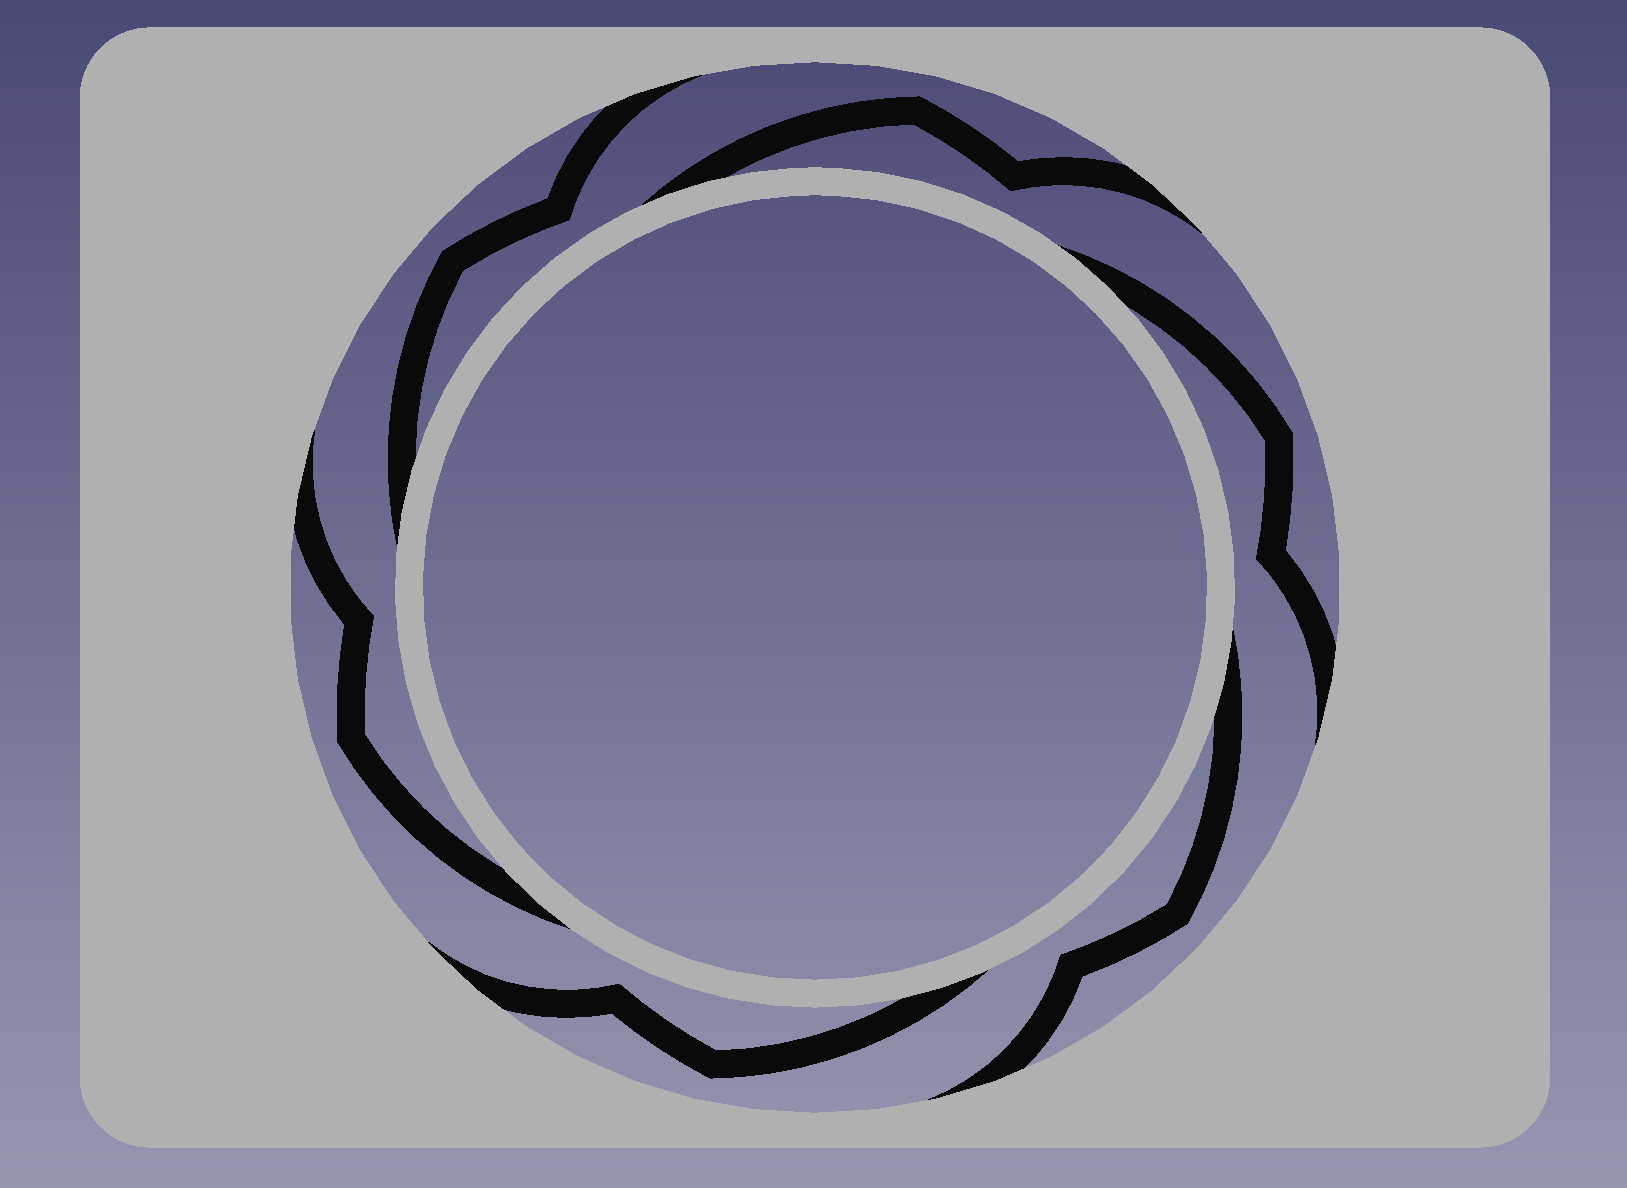
\includegraphics[width=0.9\columnwidth]{CADdesignV2}
    \caption{The final design of the RubberEdge interface used in the experiment.}
    \label{fig:cadv2}
\end{figure}

Problems occurred with the initial 3D printed design, the key of which was the spring arms breaking after a period of use. The arms broke due to them being stretched too far when the inner ring was pushed up against the wall of the outer frame. The next and final iteration of the design solved this problem by changing the spring arm design to allow the arms to extend and contract, as well as increasing the thickness of the spring arms from 1.5mm to 2mm; the final design can be seen in Figure \ref{fig:cadv2}.



\subsection{Interface Data}\label{section:interface_data}
Initially, in order to read the input from a participant using the RubberEdge device on the touchpad of a laptop the libpointing library\cite{Roussel2017Libpointing}\cite{Casiez2011NoFunctions} was used. However, after an investigation into the source code and the underlying Window's \glspl{API}\cite{RawWindows} there was no way to get the absolute position of a participants finger on the touchpad using libpointing. This is despite a method called getPosition() as part of the libpointing \gls{API}.

The authors of the reference paper used a touchpad driven by Synaptic's drivers, which could be installed on the laptop. At the time, Synaptic offered an SDK to interact with their drivers, however, it appears this is no longer offered on their website, and clones available on Github have not been kept up to date with the latest drivers.

The existing drivers on the laptop are for Windows precision touchpads. This driver provides two interfaces that a developer can subscribe to\cite{PrecisionGuide}. The first interface provides relative pointer events and is the one used by the libpointing library. The second interface positions itself as a generic touchscreen\cite{WindowsWindows}, this is used for gesture recognition and does provide the absolute coordinates for interactions with the touchpad.

Due to time constraints we were not able to use the newer driver interface, and instead found a compromise to the method of input as seen in Section \ref{section:apparatus}

